\chapter{Design}\label{ch:design}

This section discusses the design of the system. The first part explains query
spawning and execution, the second part describes how data streams can be shared
between queries.

\section{Overall Architecture}

Our system consists of multiple components which are briefly described here.
A dataflow program submitted to run as part of the system is
called a \emph{query}. Following Timely's terminology, the execution of a query
is done by a group of \emph{worker} threads. Each worker manages the scheduling and
notification of the nodes that are part instance of the dataflow graph. 

A query is executed by one or more \emph{executors}. Each executor selected to
execute a query will fetch and invoke the query binary, ultimately spawning the
worker threads. 

All these components are managed by a central process called the \emph{coordinator},
which stores the system state in the \emph{catalog}. In addition to managing
query execution, the coordinator also allows for query composition: Queries can
publish the results of their dataflow computation as \emph{topics}, which in turn
other queries can subscribe to.

\begin{table}
    \myfloatalign
  \begin{tabularx}{\textwidth}{>{\scshape}lX} \toprule
    \tableheadline{Component} & \tableheadline{Description} \\ \midrule
    Query & User-submitted Timely program running in the system.\\
    Worker & Thread belonging to a query, driving the computation of its local dataflow graph instance.  \\
    Executor & Process designated to host and spawn queries.\\
    Coordinator & Central process managing all the other components.\\
    Catalog & Data collection storing the system state at the coordinator.\\
    Topic & A named and typed representation of an exposed data stream.\\
    Publisher & Operator for exposing Timely streams by publishing them as a topic.\\
    Subscriber & Operator emitting the data stream published into a given topic.\\
    % submission
    % dataflow graph
    \bottomrule
  \end{tabularx}
  \caption{Terminology of the system}  \label{tab:design-terminology}
\end{table}


\begin{figure}[htb]
  \centering
    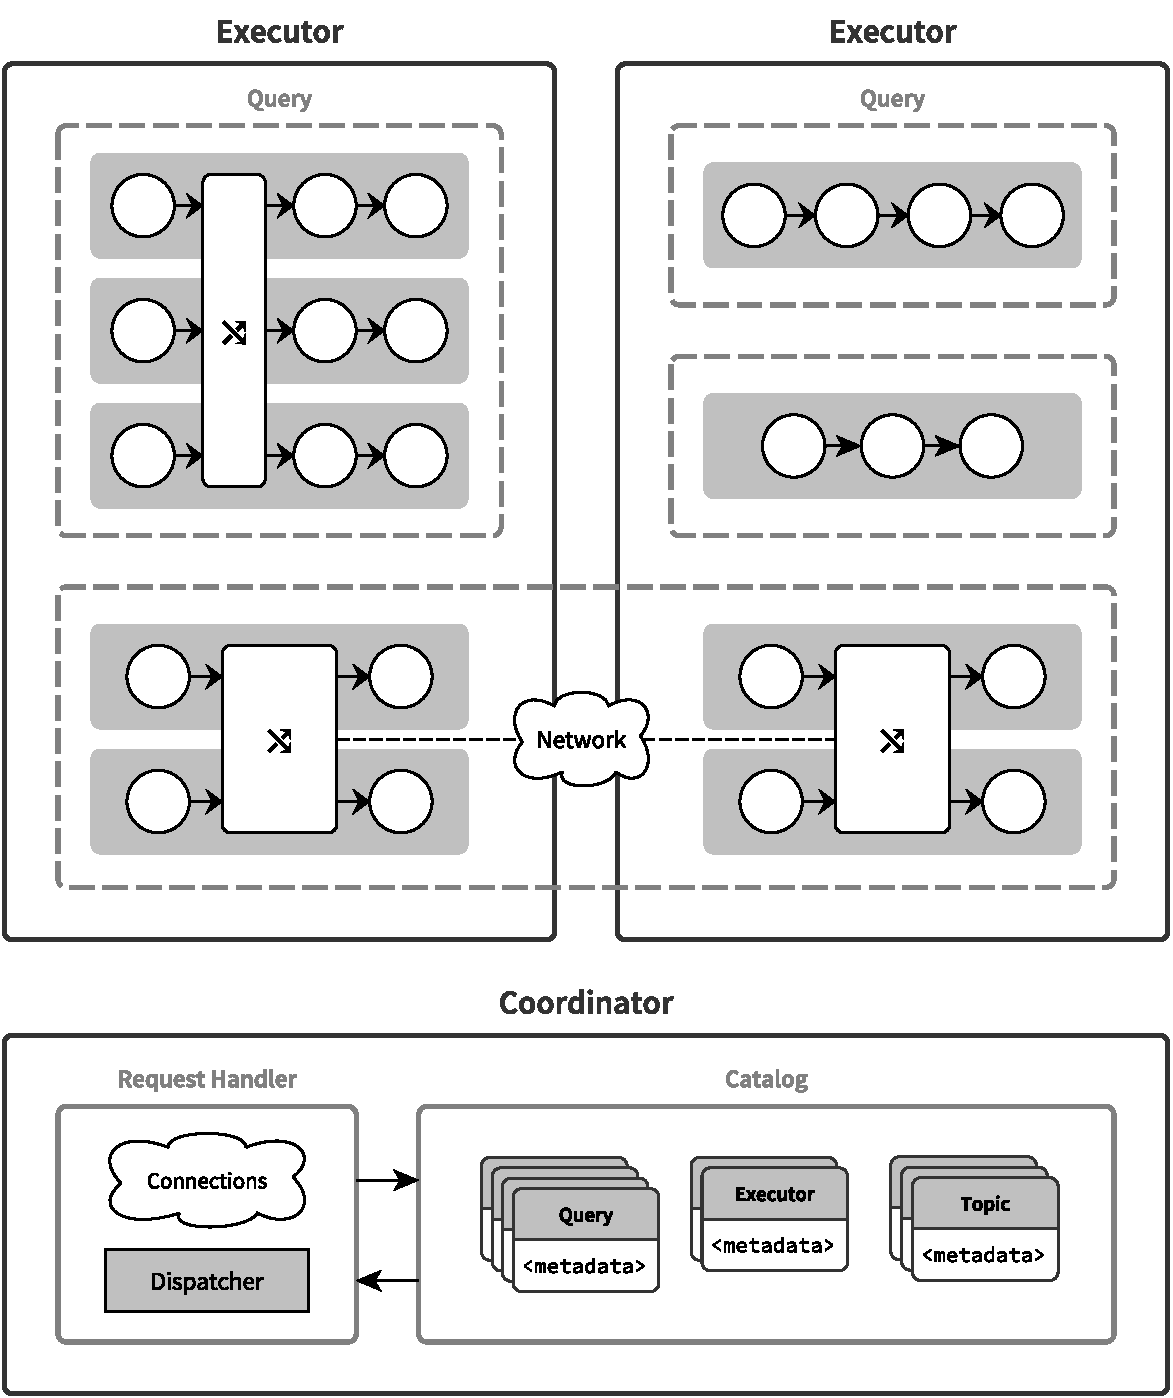
\includegraphics[width=1\textwidth]{figures/components}
  \caption[System architecture.]{ Queries (dashed boxes) consist of one or
  more worker threads (rounded grey boxes) driving the dataflow computation.
  A query might span over multiple executors, make use of the network for message exchanges
  between the workers of a query.\\
  The coordinator maintains a connection to every  executor and every query process.
  The state of the whole system is stored in the catalog.}
  \label{fig:components}
\end{figure}

\clearpage

\section{Queries}

A query is a Timely program managed and executed by our system. Like
standalone Timely Dataflow programs, queries are written in Rust by using the
Timely Dataflow library: The dataflow graph is constructed by connecting
Timely's operators (vertices) to stream objects (edges).

In order for a Timely Dataflow program to become a runnable query on the system,
it needs to register its computational logic with with our system library instead of
using Timely Dataflow's initialization function. This
\lstinline{timely_query::execute} function not only performs the initialization
for the query, it also provides additional functionality to interact with the
coordinator. Other than this, there are no restrictions on the query program,
it might execute arbitrary code. % TODO maybe rewrite

\begin{lstlisting}[caption={[Example query.]Example query which creates a stream of integers,
filters out all odd numbers and then prints the rest.}]
extern crate timely;
extern crate timely_query;

use timely::dataflow::Scope;
use timely::dataflow::operators::{Filter, Inspect, ToStream};

fn main() {
    timely_query::execute(|root, catalog| {
        root.scoped::<u32, _, _>(|scope| {
            (0..100).to_stream(scope)
                .filter(|x| x % 2 == 0)
                .inspect(|x| println!("hello {:?}", x));
        });
    }).unwrap();
}
\end{lstlisting}

Timely implements a data-parallel approach for its computation. This is done by
instantiating the dataflow graph on multiple worker threads, where each worker
drives the computation of its local instance, and the data is distributed by
user-provided sharding functions. Workers can be distributed among multiple
machines, where the computation consists of multiple operating system processes
which are communicating with each other over the network. Such an
operating system process might host multiple worker threads.

\begin{figure}[htb]
  \centering
    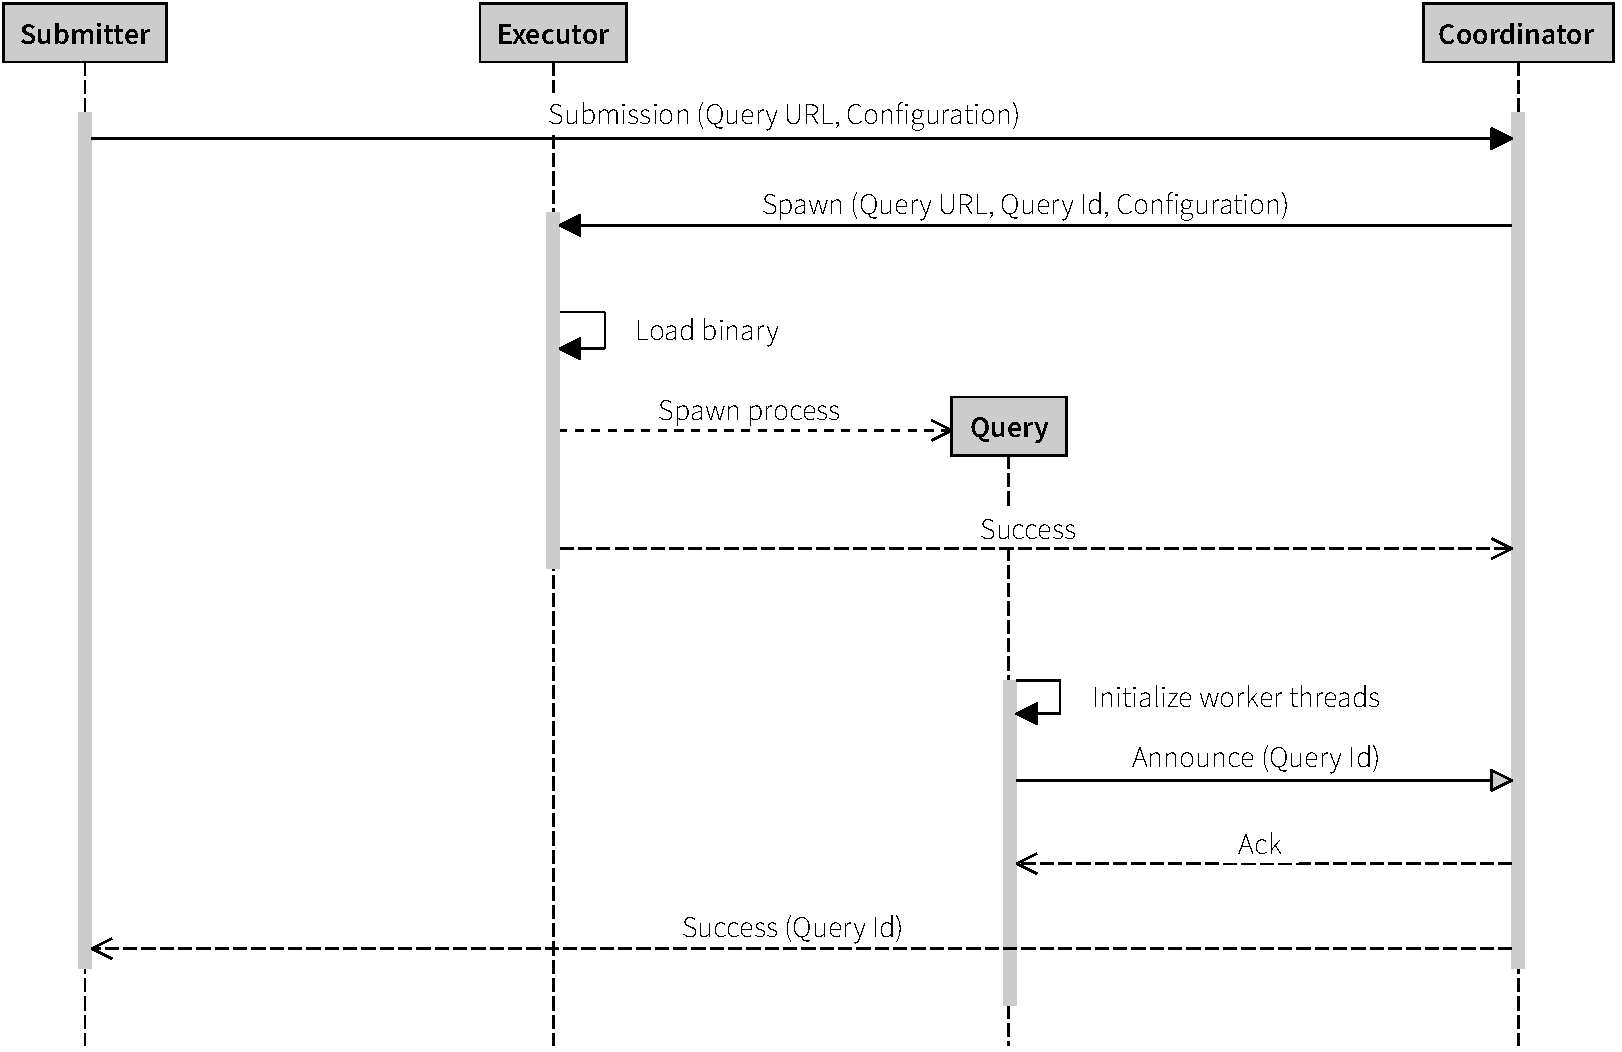
\includegraphics[width=1\textwidth]{figures/spawn_singleprocess}
  \caption[Query submission with single process.]{Submission of a query on a single executor.
  Only once the spawned query announces itself at the coordinator is it considered running.}
  \label{fig:subsingle}
\end{figure}

\section{Executors}

The spawning and direct supervision of query processes is not done by the
coordinator itself, but is offloaded to designated processes called executors.
This choice allows for more flexibility regarding query execution and the
management of available resources. Since executors can be dynamically be added
to the system, and with some limitations also be removed again, they provide
a way for adding new machines to the cluster running our system. The catalog
maintains the pool of available executors which are participating in the system.

As a timely program can span over multiple machines, a query might span
over multiple executors. The placement of a query on the available executors
is performed by the coordinator, based on the users request.
We currently implement a naive approach to query placement, where the executors
are chosen randomly if the user does not manually specify a placement. A more
sophisticated scheduling, which for example could include load balancing,
has to be investigated.

Another feature of executors are that they define on how queries and their
worker threads are supposed to be executed. When a executor joins
the system by introducing itself to the coordinator, the executor also informs
the coordinator about the execution format it supports. In the current
implementation, executors only support the execution of queries in the form of
native operating system executables.

When spawning such an executable, the newly spawned query process and the
executor coordinate. The executor supplies the newly created process with the information
it needs in order to participate in the system. This includes the query's own identifier,
the address of the coordinator, the addresses of any peer processes belonging to the 
same query, and the number of worker threads to spawn inside this process.

Executors are also responsible for fetching any query binaries they are supposed
to spawn. When submitting a new query, the submitter has to provide coordinator
with the URL of the binary. This URL is forwarded to participating executors,
which will use it to download the query binary. 

Since executors serve as a provider for computational resources such as machines,
there is typically a one-to-one mapping between executors and the machines they
are running on. This however is not a requirement of the system, the deployment of
executors is left to the user. Similarly, the user is free spawn multiple
processes belonging to the same query on the same executor if they wish to do so.

Since operating system processes can outlive their parent process, executors can
be removed from the system while the queries spawned by the executor are still
running. In this case, the coordinator removes the terminating executor from
the pool, disallowing any future queries to be hosted on the removed executor.

\paragraph{Future Work / Alternative Designs}

\TODO{Move this, and probably reformulate as well.}
Alternative executor implementations could for example host multiple queries
within the same process, by dynamically loading the query's code into an already
running process and run it on a preemptive OS thread. This would allow queries
the interchange of objects without the need for data serialization. Given
the implementation of Timely's operator scheduling, cooperative scheduling
of multiple worker threads on a single operating system thread would be
conceivable.

\section{Coordinator}

The purpose of the coordinator is to manage all components of the system. It
provides an interface for users to submit new queries and inspect the current
state of the system. In order to receive commands and report their internal state,
every executor and query process maintains a network connection to the coordinator.

Bookkeeping of the system is done by the coordinator in the catalog. The
catalog is a datastructure which contains all information about the available
executors, the running queries and their workers. 

\subsection{Submission}

A query is submitted to the coordinator as a binary executable. A submission
consists of an URL and format of the query binary, as well as the runtime
configuration for the workers. The runtime configuration specifies the amount
and distribution of the worker threads which will drive the query.

Optionally, a human-readable description of the query,
as well as the command-line arguments to be passed to the executable can be
provided. \TODO{this is currently not implemented}

When handling a new query submission request, the coordinator will assign a
unique identifier to the incoming query, and then select a
matching number of executors for the query to be spawned on. The selection
of executors is based on the runtime configuration provided by the submission
request.

The coordinator plays an important role when spawning new queries. After
issuing query spawn requests to the executors, it waits for all query processes
to register themselves at the coordinator before they begin their computation.
Only then the query is considered active and the submission request
is reported to be completed.


\section{Sharing Data Streams}

Dataflow programs typically work on streams from external sources. As the same
data source might be of interest for different dataflow computations, it seems
appropriate to also manage input data streams in our system as well. Furthermore,
input streams might not only come from external sources: A dataflow computation
might produce an intermediate or final output stream which could be of interest
for other queries. These assumptions motivate us to extend our system with a
mechanism to allow queries to expose their data streams for consumption by other
queries.

\TODO{Motivation for topic-based pubsub:

- discoverability and type-soundness of topics, type-based reflection hard

- decoupling from producer and consumer (no storing of old data, buffering done by library)

- dynamic adding and removal of topics decoupled from queries lifetime}

We loosely adapted the terminology of publish/subscribe systems: Using the
\emph{publish} operator, a query can expose one of its stream
(an edge in the dataflow graph) to other queries, which in turn then \emph{subscribe}
to it. The list of all published topics is stored at in the catalog.

\subsection{Topics}

A topic has the following properties, which are all stored in the catalog
and can be accessed by other queries.
\begin{description}
\item [Identifier] A unique identifier for the topic instance.
\item [Name] When publishing a stream, the publisher has to assign a name to it.
Queries use this name to refer to topics they want to subscribe to. There might
be only one topic with a certain name at a time, however names can be reused if
topics are unpublished.
\item [Data type] A descriptor of the data type of the stream published in this
topic. Timely's streams are typed channels, therefore so are topics.
\item [Address] An address to which the subscribers connect in order to received
the contents of the published stream.
\end{description}

While every publication and subscription request is disclosed to the coordinator
and the catalog contains a list of all existing topics, the
actual exchange of data happens directly between queries. When a query subscribes
to a topic, it receives the address of the topic's publisher from the coordinator
and directly connects to it.

\subsection{Stream Publisher}

A stream publisher is a Timely operator which exposes a Timely stream as a topic. When
creating it, the query author has to assign a name for the topic under which the
input stream will be published. As with all other Timely operators, the publisher
operator is instantiated on all worker threads. However, the user can choose
whether all worker streams are merged into a single topic before publishing, or
if each worker publishes its own topic. The latter option implicitly exposes
the data sharding strategy of the publishing query, allowing the workers of
the subscribing query to exploit this partition scheme.

\subsubsection{Collection Publisher}

\begin{comment}
This however might be too limiting for some use cases where previously published
data might is essential for a full understanding of the data stream. A simple
solution for this problem would be to buffer the stream at the publisher
and replay it to every incoming subscriber. While simple, this approach
would be wasteful in cases where the data in the buffer becomes stale and
irrelevant to future subscribers. \TODO{this doesn't motivate \emph{unordered}
multisets}
\end{comment}

Normally, publishers are not buffered, meaning subscribers will
not receive any data which was produced before they subscribed to a certain
topic. This is the same as in many other publish/subscribe systems, where
synchronization between publishers and subscribers is decoupled as well. \cite{pubsub}

However, in streams where the contents of the stream describes changes of a certain
state, it is essential for stream consumers to know the state of the source at
the beginning of the stream in order to make sense out of it.

For this reason, we introduce a different kind of publisher which publishes
\emph{collections} instead of streams. A collection is a typed, unordered
multiset maintained by the publisher, possibly representing state it would
like to share with subscribers.

Upon creation, a collection publisher contains an empty collection.
When the publishing query mutates the collection by adding or removing elements,
these changes are propagated to the subscribers. When new subscribers connect
to this publisher, they will initially receive a list of all currently contained
elements. This way, all subscribers eventually maintain the same view of the
data collection.

From the subscribers point of view, a topic published by a collection publisher
is not inherently different from a normal topic: After subscribing, it will
observe a continuous stream of data. The difference is in the data type of the
stream, it will be of tuples of the format $(\texttt{Data}, \delta)$, where
\texttt{Data} is an element that can be stored in the multiset and $\delta$ 
denotes the amount of elements that have been added or removed from the set.
This format
is compatible with the notion of collections in Differential Dataflow, allowing
subscribing queries to further process the collection in a convenient manner.

\subsection{Subscriber}

In order to subscribe to a topic, the subscribing query has to provide the name
of the topic it is interested in. This involves a name lookup which can optionally
be blocking: If a requested topic does not yet exist, the coordinator will add
the subscriber to a wait list. Once a corresponding topic is published under that
name, the coordinator will inform the subscriber about this topic. 

The subscribing query might use different timestamps in its dataflow graph
than the publisher, thus it is the subscribers responsibility to re-add
timestamps to the received stream. 

\subsection{Alternative Approaches}

\subsubsection{Capture \& Replay Operator}

The Timely library also offers the capture and replay operators which serve the
purpose of sharing data between queries. With the capture operator, all timestamp,
data and event records are collected and stored in one dataflow computation,
and can then be replayed in another one.

The implementation of the replay operator requires it to use the same timestamps
as the capture operator, forcing both queries to have a similar structure
in their dataflow graph, as a timestamp received at an operator is defined
by its surrounding scope. Another feature of the capture/replay operator pair
is that they will replay the whole stream from beginning to end, requiring the
capture operator to either buffer its incoming data or wait for the replaying
query to connect to it. 

Both these requirements stem from the fact that the replay operator not only
replays the data stream, but also all progress tracking events, including
notifications. In our system, we opted for a more dynamic approach, where
producing queries are allowed to discard data if there are no consumers, and
where consumers use the streams as inputs for their own computation,
allowing them to assign their own timestamps to the data stream.

It is the user's task to provide a communication channel between capture and 
replay operators. Common channel include Rust's thread-safe FIFO queues or
TCP sockets. In general it can be said the capture/replay operators result
in a more tightly coupled system than publish/subscribe pairs.


\subsubsection{Retroactive Tapping of Dataflow Edges}
\begin{addedbar}
With the current publish/subscribe mechanisms, query authors are required to
anticipate which operator outputs are of possible interest for subscribers. If
a certain output is not explicitly published using the publish operator, there
is no way for other queries to access it.

 tap into arbitrary operator outputs and publish them as topics
upon request.

The design choice of topics as streams that can be dynamically added or removed
from the catalog was made with such a use-case in mind. However, due to the fact
that timely decouples message delivery from operator scheduling (see
\fullref{sec:runtime-graph}), workers do not maintain a central registry of which
queue belongs to which operator. As a consequence, outside access to the output of
a given operator would only be possible with modifications to Timely, which was
not in the scope of the remaining time.

\end{addedbar}
